\chapter{Experiments and Results}
\label{ch:experiments}

This chapter reports the empirical evaluation of the framework developed in
Chapter~\ref{ch:methodology}. The experiments are organised to mirror the four
research contributions of Section~\ref{sec:celePracy}:
Section~\ref{sec:exp-setup} fixes the experimental configuration;
Section~\ref{sec:exp-redundancy} presents the metric redundancy analysis
(Contribution~1); Section~\ref{sec:exp-meta} reports the meta-evaluation of
metric reliability (Contribution~2); Section~\ref{sec:exp-ranking} compares the
uniform, Autoweighted, and MetaQuantus-discounted aggregation schemes
(Contributions~2--3); Section~\ref{sec:exp-ensemble} contrasts individual and
NormEnsembleXAI-ensembled attributions (Contribution~3); and
Section~\ref{sec:exp-stats} establishes statistical significance via Friedman,
Nemenyi, and Wilcoxon testing (Contribution~4).

All quantitative tables in this chapter are generated directly from the
result artifacts under \texttt{results/} by
\texttt{experiments/render\_results\_tables.py} and \texttt{\textbackslash
input}-ed here. The scores, rankings, ensemble comparison, and statistical
tests are computed over the full 600-image ISIC~2017 test split; the
meta-evaluation (Section~\ref{sec:exp-meta}) is the deliberate exception,
running on a fixed 64-image sample, as disclosed where its numbers are used.
Two further
limitations are stated up front and revisited at the
point of use: (i)~both reliability legs of the two $M^{*}$
metrics that internally re-compute attributions (\emph{max\_sensitivity},
\emph{random\_logit}) come from repaired follow-up runs: their original
Noise-Resilience measurements failed silently and were re-measured with a
fixed estimator, and scoring their AR required an extension
of the AR protocol---the
degradation is injected into the explanation function itself
(Section~\ref{sec:exp-meta}). With both repairs every $M^{*}$ metric
carries a fully measured reliability, and the MQ-discount genuinely
reweights the index (mean $|\Delta|\approx0.14$ on ResNet-18 and $0.06$ on
SqueezeNet relative to Autoweighted,
with a model-dependent effect on the ranking); and (ii)~the attribution-ensembling
experiment of Section~\ref{sec:exp-ensemble} ensembles \emph{all seven}
methods, Occlusion included---the generating notebook passes the full
method registry to NormEnsembleXAI (an earlier draft of this chapter
mis-stated a six-gradient ensemble)---and uses the full 600 images and all
seven $M^{*}$ metrics.
Cells reading \textit{n/a} denote a value
that is genuinely undefined (e.g.\ a single-metric category has no
within-category correlation), not a missing computation.

%% ========================================================================
\section{Experimental Setup}
\label{sec:exp-setup}

\subsection{Data and Splits}

All experiments use the ISIC~2017 Challenge dataset (Task~1) described in
Section~\ref{sec:dataset}: 2{,}000 training, 150 validation, and 600 test
dermoscopic images across three diagnostic classes (melanoma, nevus,
seborrheic keratosis), each paired with an expert-annotated binary lesion
mask. The redundancy, aggregation, and statistical analyses are computed on
the full 600-image test split; the meta-evaluation runs on a fixed 64-image
sample (Section~\ref{sec:exp-meta}). A fixed, reproducible
12-image pilot subset of the test split was used to validate the pipeline
plumbing prior to the full run; Table~\ref{tab:exp-scale} contrasts the two
scales.

\subsection{Models}

Two classifiers act as the predictors whose decisions are explained: ResNet-18
(final \texttt{fc}~$\to$~\texttt{Linear(512, 3)}) and SqueezeNet~1.1 (final
classifier~$\to$~\texttt{Conv2d(512, 3, 1, 1)}). Both are trained with the
protocol of Section~\ref{sec:models} (25 epochs, SGD with momentum,
class-weighted cross-entropy, StepLR, fixed seed~42). Validation accuracy and
trained-weight checksums are reported in Table~\ref{tab:model-summary}.

\begin{table}[H]
\centering
\caption{Predictive models under evaluation and their training outcome.
Best validation accuracy is taken from the 25-epoch training logs; test-set
accuracy is marked \textit{n/a} as the 600-image test split was used for
explanation evaluation (with the model's own prediction as the attribution
target), not for separate classification scoring.}
\begin{tabularx}{\linewidth}{llcc}
\toprule
Model & Head & Best val.\ accuracy & Test accuracy \\
\midrule
ResNet-18      & Linear(512, 3)        & 75.3\% & \textit{n/a} \\
SqueezeNet 1.1 & Conv2d(512, 3, 1, 1)  & 74.0\% & \textit{n/a} \\
\bottomrule
\end{tabularx}
\label{tab:model-summary}
% Source: results/training_log_{resnet18,squeezenet}.csv (full ISIC 2017,
% 25 epochs, 2026-04-22) and weights/README.md — final weights, not pilot.
\end{table}

\subsection{Attribution Methods}

Seven FAE methods are evaluated (Section~\ref{sec:fae-methods}): Saliency,
Integrated Gradients, Grad-CAM, Guided Backpropagation, DeepLift, LRP
(gradient-based), and Occlusion (perturbation-based). LIME and KernelSHAP were
excluded from the experiment for runtime reasons, as discussed in
Section~\ref{subsec:excluded-fae}.

\subsection{Metrics, Hardware, and Reproducibility}

The twelve metrics of Table~\ref{tab:metrics} are computed with the
hyperparameters listed there. Reproducibility rests on three committed
artifacts rather than declarative configuration files: the Colab notebooks
that produce the raw scores (with seeds and metric hyperparameters fixed in
code and the Quantus version pinned), the raw per-(model, image, FAE,
metric) score table itself
(\texttt{results/full\_run\_7fae\_12metrics\_600.csv}; the pilot counterpart
is \texttt{results/vertical\_slice\_7fae\_12metrics.csv}), and the
post-processing scripts under \texttt{experiments/}, which regenerate every
table in this chapter deterministically from that score table (the full
package environment is recorded in \texttt{requirements-lock.txt}). The
expensive GPU stage is thus re-runnable from the notebooks and auditable
from the committed scores, but it is not driven by a single declarative
configuration file.

\begin{table}[H]
\centering
\caption{Experiment scale: pilot vs.\ full run.}
\begin{tabularx}{\linewidth}{lcc}
\toprule
Quantity & Pilot & Full run \\
\midrule
Test images        & 12  & 600 \\
Models             & 2   & 2 \\
FAE methods        & 7   & 7 \\
Metrics            & 12  & 12 \\
Score rows         & 2{,}016 & 100{,}800 \\
\bottomrule
\end{tabularx}
\label{tab:exp-scale}
% Full-run row count verified: 2 models x 7 FAE x 600 images x 12 metrics
% = 100,800 rows in results/full_run_7fae_12metrics_600.csv.
\end{table}

%% ========================================================================
\section{Metric Redundancy Analysis (Contribution~1)}
\label{sec:exp-redundancy}

This section addresses whether the twelve metrics carry independent signal or
duplicate one another. Following Decision~D4, for each model the metrics are
first variance-pre-screened (a metric is dropped if, within a model group, the
non-NaN fraction falls below 0.20 or the standard deviation falls below
$10^{-6}$), then the Spearman rank-correlation matrix is computed across the
test images, and pairs with $|\rho| > 0.85$ are greedily pruned, retaining in
each pair the metric less correlated with the remainder. The surviving set is
the reduced, non-redundant subset $M^{*}$ that feeds the aggregation stage.

\paragraph{Pre-screen.}
Two metrics are removed before correlation analysis on structural grounds:
\emph{Completeness} (constant across all applicable samples, hence
zero-variance and uninformative for ranking; see Table~\ref{tab:axiom} for
what that constant means) and \emph{Non-Sensitivity}
(disabled by default due to $O(d)$ forward-pass cost); \emph{MPRT} was
disabled for the full run outright (Section~\ref{sec:metrics}). The
remaining nine
metrics enter the matrix.

\paragraph{Correlation matrices.}
Tables~\ref{tab:redundancy-resnet} and~\ref{tab:redundancy-squeeze} hold the
within-category redundancy summaries for ResNet-18 and SqueezeNet, derived from
\texttt{results/redundancy\_matrix\_resnet18.csv} and
\texttt{results/redundancy\_matrix\_squeezenet.csv}. The full $9 \times 9$
Spearman matrices are reproduced in those CSVs; only the summary and the pruned
pairs are shown here for legibility.

% Auto-generated by experiments/render_results_tables.py — do not edit.
% Regenerate after each run; \input this file from chapter4_state_observers.tex.
\begin{table}[H]
\centering
\caption{Redundancy summary --- ResNet-18: within-category mean $|\rho|$ at
the $|\rho| > 0.85$ pruning threshold (pilot, 12 images).}
\begin{tabularx}{\linewidth}{lcc}
\toprule
Category & $n$ metrics & Mean $|\rho|$ \\
\midrule
Complexity & 2 & 0.997 \\
Robustness & 2 & 0.929 \\
Randomization & 2 & 0.829 \\
Localization & 2 & 0.180 \\
Faithfulness & 2 & 0.011 \\
\bottomrule
\end{tabularx}
\label{tab:redundancy-resnet}
\end{table}


% Auto-generated by experiments/render_results_tables.py — do not edit.
% Regenerate after each run; \input this file from chapter4_state_observers.tex.
\begin{table}[H]
\centering
\caption{Redundancy summary --- SqueezeNet~1.1: within-category mean $|\rho|$ at
the $|\rho| > 0.85$ pruning threshold (pilot, 12 images).}
\begin{tabularx}{\linewidth}{lcc}
\toprule
Category & $n$ metrics & Mean $|\rho|$ \\
\midrule
Complexity & 2 & 0.991 \\
Robustness & 2 & 0.969 \\
Randomization & 2 & 0.709 \\
Localization & 2 & 0.312 \\
Faithfulness & 2 & 0.003 \\
\bottomrule
\end{tabularx}
\label{tab:redundancy-squeeze}
\end{table}


\paragraph{Pruning outcome and $M^{*}$.}
On the full 600-image run the Complexity pair (complexity / sparseness,
$|\rho| \approx 0.99$ on both models) and the Robustness pair
(avg-/max-sensitivity, $|\rho| \approx 0.93$ on ResNet-18 and $0.98$ on
SqueezeNet) are strongly redundant, whereas the Faithfulness and Localization
pairs are nearly orthogonal ($|\rho| < 0.25$ in every case). The greedy
$|\rho| > 0.85$ pruning therefore drops one metric from each redundant pair
in both models (complexity in favour of sparseness; avg-sensitivity in favour
of max-sensitivity). The resulting reduced set $M^{*}$ is \emph{identical} for
the two models and comprises the same seven metrics:
\emph{faithfulness\_correlation}, \emph{max\_sensitivity},
\emph{pixel\_flipping}, \emph{pointing\_game}, \emph{random\_logit},
\emph{relevance\_mass\_accuracy}, and \emph{sparseness}
(Tables~\ref{tab:redundancy-resnet}--\ref{tab:redundancy-squeeze}). That the
two architectures yield the same $M^{*}$ is the principal evidence for
Contribution~1: the redundancy structure of these metrics is shared across
the two studied classifiers rather than idiosyncratic to either---evidence
of consistency under these conditions, not proof of general
classifier-independence. One caveat on that identity
deserves disclosure: within the Complexity pair on ResNet-18 the greedy rule
retains sparseness over complexity by a razor-thin margin (mean
$|\rho|$-with-the-remainder of $0.323$ vs.\ $0.325$). An image-level
bootstrap addresses whether that margin makes the result fragile: across
$200$ resamples of the $600$ test images (with replacement, per model;
\texttt{experiments/bootstrap\_mstar.py}, seed 42), the pruned set equals
the reported $M^{*}$ in $200/200$ replicates on both models, and the
cross-model identity holds in $200/200$---the tie-break margin is thin, but
the selection is empirically stable under resampling of this test split.
The pruning costs no
discriminative signal in practice: the per-method mean-effectiveness ranking
computed over the full nine-metric battery and over $M^{*}$ (uniform
weights) are identical on both models (Spearman $\rho = 1.00$).
Table~\ref{tab:mstar} records
the set carried forward into aggregation.

\begin{table}[H]
\centering
\caption{Reduced metric set $M^{*}$ after redundancy pruning (full run, 600
images). The set is identical for both models.}
\begin{tabularx}{\linewidth}{lX}
\toprule
Set & Metrics retained \\
\midrule
ResNet-18 (7)     & f\_corr, max\_sens, pixel\_flip, point\_game, rand\_logit, RMA, sparseness \\
SqueezeNet (7)    & f\_corr, max\_sens, pixel\_flip, point\_game, rand\_logit, RMA, sparseness \\
Intersection (7)  & f\_corr, max\_sens, pixel\_flip, point\_game, rand\_logit, RMA, sparseness \\
\bottomrule
\end{tabularx}
\label{tab:mstar}
\end{table}

\begin{table}[H]
\centering
\caption{Completeness indicator (Quantus, strict float equality; full run,
$n = 600$ per cell). Quantus returns a per-sample Boolean --- $1$ if the
attribution sum equals $f(x) - f(x')$ \emph{exactly} --- and that strict
equality never holds in floating point, so the indicator is uniformly
$0$ (False). An earlier draft of this table inverted the Boolean's
semantics and reported the constant $0$ as a perfect pass; the corrected
reading is that the strict-equality indicator can neither confirm nor
refute the axiom at machine precision, and a tolerance-based verification
of the underlying sums was not performed. Either way the column is
constant, which is what the pre-screen acts on.}
\begin{tabularx}{\linewidth}{llcc}
\toprule
Model & FAE method & Indicator (all samples) & Strict-equality pass \\
\midrule
ResNet-18 / SqueezeNet & Integrated Gradients & 0 & No \\
ResNet-18 / SqueezeNet & DeepLift             & 0 & No \\
ResNet-18 / SqueezeNet & LRP                  & 0 & No \\
\bottomrule
\end{tabularx}
\label{tab:axiom}
% Source: results/axiom_verification.csv (corrected semantics, 2026-08-28:
% expected value = 1.0/True; all six cells fail strict equality on all 600).
\end{table}

%% ========================================================================
\section{Meta-Evaluation: Metric Reliability (Contribution~2)}
\label{sec:exp-meta}

The redundancy analysis identifies which metrics overlap; meta-evaluation
identifies which metrics can be \emph{trusted}. Each metric in $M^{*}$ is
subjected to this thesis's estimators of the two MetaQuantus reliability
properties (Section~\ref{subsec:mq-discount}): Noise Resilience (NR),
measuring score
stability under semantically meaningless input/weight perturbation, and
Adversarial Reactivity (AR), measuring whether the score reacts
systematically as
the explanation is deliberately degraded. The combined reliability
$r_k = \tfrac{1}{2}(\mathrm{NR}_k + \mathrm{AR}_k)$ is the discount coefficient
used in Equation~\eqref{eq:mq-discount}.

Unlike every other analysis in this chapter, the meta-evaluation runs on a
fixed, seed-determined \textbf{64-image random sample} of the test split per
(model, FAE) cell (5 noise seeds, 5 degradation levels); the extended-AR
completion for \emph{max\_sensitivity} and \emph{random\_logit} runs on the
\textbf{same 64-image sample} at a finer 10-level degradation grid, so every
$M^{*}$ metric's reliability rests on a single sample. One protocol
deviation on that sample must be disclosed: the meta-evaluation's
attribution targets were computed once from ResNet-18's predictions and
supplied to \emph{both} models, whereas the main scoring run uses each
model's own prediction (Section~\ref{sec:metrics}); the two models disagree
on 25 of the 64 sampled images, so SqueezeNet's reliability cells were
evaluated at the ResNet-18-predicted class on those images. Because NR and
AR characterise the \emph{metric's} stability and reactivity at a fixed
target rather than the model's correctness, the reliability estimand is
arguably robust to this choice, but re-running the SqueezeNet
meta-evaluation with its own targets is listed as future work. The
reliability
estimates are in any case
coarse, and are treated as such: values are reported to two decimals, the
between-cell dispersion is reported alongside each mean, and the
robustness of the downstream MQ-discount finding to these estimates is
checked below.

\paragraph{A silent failure in the NR stage, and its correction.}
An independent audit of the reliability data found that the Noise-Resilience
values originally recorded for the explanation-recomputing metrics
(\emph{max\_sensitivity}, \emph{avg\_sensitivity}, \emph{random\_logit})
were $1.00$ \emph{bitwise-identically} in all 14 (model, FAE) cells---while
every metric that demonstrably computed shows between-cell variation. The
cause was a defect in the NR implementation: when every seeded metric call
fails (as those metrics' calls did in the original meta-evaluation run,
consistent
with their near-uniform per-cell runtimes and their simultaneously
unmeasurable AR), the empty score set produced a coefficient of variation of
zero and thus a ``perfect'' $\mathrm{NR}=1.0$---total failure scored as
total stability. The defect was fixed (failed measurements now
yield NaN), the artifact values were discarded, and NR for the two $M^{*}$
metrics was \emph{re-measured} on the same 64-image sample with the
repaired estimator; the values in Table~\ref{tab:meta} are those
re-measurements, with genuine between-cell variation
($\mathrm{NR} \in [0.56, 1.00]$ for max\_sensitivity). Every reliability
number that enters the discount is therefore a real measurement.

Table~\ref{tab:meta} reports NR, AR, and combined reliability per metric,
averaged over the (model, FAE) cells in which each metric is defined, read from
\texttt{results/meta\_evaluation\_reliability.csv}. The runtime
column documents the meta-evaluation cost per cell at these sample sizes
(the full-run evaluation cost per metric is substantially larger and scales
with the 600-image split).

% Auto-generated by experiments/render_results_tables.py — do not edit.
% Regenerate after each run; \input this file from chapter4_state_observers.tex.
\begin{table}[H]
\centering
\caption{Metric reliability from MetaQuantus (NR, AR, combined), averaged over
(model, FAE) cells. Cells marked \textit{n/a} are metrics whose Adversarial
Reactivity could not be scored in this run (the \texttt{explain\_func}-based
perturbation failed), so no combined reliability is available.}
\begin{tabularx}{\linewidth}{lcccc}
\toprule
Metric & NR & AR & Combined $r_k$ & Mean runtime (s) \\
\midrule
faithfulness\_correlation & 0.564 & 0.600 & 0.582 & 151.5 \\
max\_sensitivity & 1.000 & \textit{n/a} & \textit{n/a} & 128.2 \\
pixel\_flipping & 0.995 & 0.771 & 0.883 & 186.7 \\
pointing\_game & 0.962 & 0.659 & 0.811 & 40.7 \\
random\_logit & 1.000 & \textit{n/a} & \textit{n/a} & 127.2 \\
relevance\_mass\_accuracy & 0.589 & 0.514 & 0.552 & 40.5 \\
sparseness & 0.994 & 0.943 & 0.969 & 40.4 \\
\bottomrule
\end{tabularx}
\label{tab:meta}
\end{table}


The reliability table is read as follows: a metric with high NR but low AR is
stable but insensitive (it does not react when the explanation degrades); a
metric with low NR is noisy. Among the $M^{*}$ metrics, \emph{sparseness}
($r_k = 0.97$), \emph{max\_sensitivity} ($0.96$), and
\emph{pixel\_flipping}
($0.88$) are the most reliable; \emph{pointing\_game} ($0.81$) follows.
\emph{Random\_logit} ($r_k = 0.63$) is the textbook case of the
stable-but-insensitive pattern: its NR is near-perfect ($0.99$) while its
measured reactivity sits at the noise floor
(below). \emph{Faithfulness\_correlation}
($0.58$) and
\emph{relevance\_mass\_accuracy} ($0.55$) also score low: both are
noise-resilient only moderately (NR $\approx 0.56$--$0.59$) and react
comparatively weakly to deliberate degradation (AR $\approx 0.51$--$0.60$).
The dispersion column tempers these point estimates: the least reliable
metrics are also the least consistently estimated
($\mathrm{SD}(r_k) = 0.28$ for faithfulness\_correlation, whose per-cell
values span $0.05$--$0.98$), whereas the most
reliable metrics are also the
most stable across cells ($\mathrm{SD} \approx 0.09$--$0.15$).

Two audits qualify the AR leg. First, because AR is the \emph{absolute}
Spearman correlation, a metric reacting in the unexpected direction would
still earn credit; auditing the signed monotonicity of the 28 extended-AR
cells finds one such cell (\emph{random\_logit} on
guided-backprop/ResNet-18, $|\rho_S| = 0.59$) --- its contribution is
disclosed rather than re-scored, and a direction-rectified AR is noted as
future work. Relatedly, \emph{random\_logit}'s mean AR of $0.27$ sits at
the noise floor of a ten-point $|\rho_S|$ estimate (the expected
$|\rho_S|$ of a random ordering over ten levels is ${\approx}0.27$, and
$45\%$ of random orderings exceed the measured value), and its per-cell
signed monotonicity is mixed (9 of 14 cells positive): its measured
adversarial reactivity is statistically indistinguishable from zero, so
its combined $r_k = 0.63$ is carried almost entirely by its
noise resilience.
\emph{Max\_sensitivity}, by contrast, is overwhelmingly directional (13 of
14 cells positive, mean signed $\rho_S = 0.91$)---a real, if partly
mechanical, response (see Section~\ref{sec:disc-threats}). Second, a
leave-one-cell-out jackknife of the per-metric
$\lambda_k$ (recomputing the MQ-discounted ResNet-18 ranking with each of
the seven FAE cells removed from the reliability average) preserves the
top-2 \emph{set} in all seven replicates: LRP and Occlusion occupy the top
two places in every replicate, but their mutual order flips (the two sit
within $0.001$ at the point estimate), and shifting the two
extension-measured reliabilities by $\pm 0.2$ likewise preserves LRP in
the top two while reshuffling its companion. At the bottom, Grad-CAM is
last at the point estimate but within $0.003$ of DeepLift and Guided
Backpropagation---a cluster, not a resolved order. The robust statement
is therefore that the discount lifts LRP from fifth under Autoweighted
into a statistical tie with Occlusion at the top, and drops Grad-CAM from
the uniform-weighting podium into the bottom cluster, while neither the
exact winner nor the bottom-three order should be over-read.

\paragraph{Extending AR to explanation-recomputing metrics.}
The MetaQuantus AR protocol degrades the explanation by zeroing a growing
fraction of the attribution array. Two $M^{*}$ metrics ignore that array:
\emph{max\_sensitivity} and \emph{random\_logit} re-compute attributions
internally through \texttt{explain\_func}, so the array degradation never
reaches them and their AR was initially unmeasurable (an earlier run of this
pipeline reported \textit{n/a} for both). The AR test was therefore
extended: for such metrics the degradation is additionally injected into the
explanation function itself---each invocation zeroes a fresh random fraction
of the explainer's output, so the metric's internal re-explanations lose
signal at the same rate as the explicit attribution (degradation capped at
$0.9$, since a fully zeroed attribution is rejected by the metric
implementations). With this extension, every computable metric carries a
combined reliability ($126$ of $168$ reliability rows are valid; the
remaining $42$ belong to the three structurally excluded metrics---MPRT,
Non-Sensitivity, and the constant-indicator Completeness). The completed
discount
is far from a no-op: it shifts the effectiveness magnitudes by mean
$|\Delta|\approx0.14$ on ResNet-18 and $0.06$ on SqueezeNet relative to
Autoweighted, and reorders the ResNet-18
field substantially ($\rho(\mathrm{AW},\mathrm{MQ}) = 0.46$; LRP rises from
fifth under Autoweighted into a statistical tie with Occlusion at the
top) while altering
SqueezeNet only mildly
($\rho = 0.96$;
Table~\ref{tab:rank-stability}).

%% ========================================================================
\section{Aggregation and Ranking Comparison (Contributions~2--3)}
\label{sec:exp-ranking}

This section measures whether \emph{how} metrics are combined changes the
conclusion about which FAE method is best. Three weighting schemes are applied
to the same normalised scores over $M^{*}$:
(i)~\textbf{uniform} ($w_k = 1/|M^{*}|$);
(ii)~\textbf{Autoweighted} (inverse-coefficient-of-variation weights,
Equation~\eqref{eq:autoweighted});
(iii)~\textbf{MQ-discounted} (Equation~\eqref{eq:mq-discount}, the
Autoweighted weights attenuated by reliability). A single-metric baseline
(Faithfulness Correlation
alone, \texttt{effectiveness\_single\_fc}) is included to quantify how far a
naive one-metric ranking departs from the multi-criteria index. All four columns
are present in \texttt{results/ranking\_comparison.csv}. As noted in
Section~\ref{sec:exp-meta}, the MQ-discount column applies a genuine
reliability reweighting (mean $|\Delta|\approx0.14$ on ResNet-18, $0.06$ on
SqueezeNet, relative to Autoweighted):
it reorders the ResNet-18 field substantially ($\rho = 0.46$) while altering
SqueezeNet only mildly ($\rho = 0.96$). The de-facto weight vectors that
produce this are disclosed here because they qualify every aggregate in
this section: under Autoweighted-with-discount on ResNet-18 the index is
dominated by sparseness ($w = 0.45$) and random-logit ($0.23$), with
pixel-flipping at $0.17$, pointing-game at $0.13$, and---owing to the
location-sensitivity of the inverse-CV weight documented in
Section~\ref{sec:weighting}---faithfulness-correlation at only $0.02$,
max-sensitivity at $0.006$, and
relevance-mass-accuracy at effectively zero. The ``multi-criteria'' index
under these data-adaptive schemes is thus in practice a three-to-four
metric index; note also that random-logit retains the second-largest
weight despite its heavily discounted $\lambda_k$, because the
multiplicative discount can only rescale the large Autoweighted allocation
it starts from. The comparison against the Single-FC baseline below
should be read with FC's near-zero weight in the index in mind.

% Auto-generated by experiments/render_results_tables.py — do not edit.
% Regenerate after each run; \input this file from chapter4_state_observers.tex.
\begin{table}[H]
\centering
\caption{Mean effectiveness index $E(\Phi)$ per FAE method under each weighting
scheme (ResNet-18, averaged over test images).}
\begin{tabularx}{\linewidth}{lcccc}
\toprule
FAE method & Uniform & Autoweighted & MQ-discount & Single-FC \\
\midrule
integrated\_gradients & 0.030 & -0.235 & -0.334 & 0.220 \\
saliency & 0.130 & -0.080 & -0.161 & 0.362 \\
gradcam & 0.274 & -0.012 & -0.111 & 0.844 \\
guided\_backprop & -0.258 & -0.596 & -0.718 & 0.042 \\
deep\_lift & -0.104 & -0.339 & -0.417 & 0.164 \\
lrp & -0.307 & -0.575 & -0.674 & -0.081 \\
occlusion & 0.220 & 0.044 & -0.034 & 0.580 \\
\bottomrule
\end{tabularx}
\label{tab:ranking-resnet}
\end{table}


% Auto-generated by experiments/render_results_tables.py — do not edit.
% Regenerate after each run; \input this file from chapter4_state_observers.tex.
\begin{table}[H]
\centering
\caption{Mean effectiveness index $E(\Phi)$ per FAE method under each weighting
scheme (SqueezeNet, averaged over test images).}
\begin{tabularx}{\linewidth}{lcccc}
\toprule
FAE method & Uniform & Autoweighted & MQ-discount & Single-FC \\
\midrule
integrated\_gradients & -0.189 & -0.033 & 0.018 & -0.025 \\
saliency & -0.001 & 0.058 & 0.102 & 0.718 \\
gradcam & 0.142 & 0.124 & 0.162 & 1.435 \\
guided\_backprop & -0.127 & -0.004 & 0.060 & 0.096 \\
deep\_lift & -0.205 & -0.058 & -0.005 & 0.019 \\
lrp & -0.189 & -0.037 & 0.015 & -0.083 \\
occlusion & 0.086 & 0.066 & 0.084 & 1.166 \\
\bottomrule
\end{tabularx}
\label{tab:ranking-squeeze}
\end{table}


% Auto-generated by experiments/render_results_tables.py — do not edit.
% Regenerate after each run; \input this file from chapter4_state_observers.tex.
\begin{table}[H]
\centering
\caption{Induced FAE-method ranks under each weighting scheme, and
rank-stability summary (Spearman rank correlation between per-method mean-$E$
rankings; rank inversions summed over both models).}
\begin{tabularx}{\linewidth}{lcccc}
\toprule
Comparison & Uniform vs.\ AW & Uniform vs.\ MQ & AW vs.\ MQ & Single-FC vs.\ MQ \\
\midrule
Spearman rank corr.\ (ResNet-18)  & 0.929 & 0.929 & 1.000 & 0.929 \\
Spearman rank corr.\ (SqueezeNet) & 0.857 & 0.929 & 0.964 & 0.679 \\
\# rank inversions                & 5 & 4 & 1 & 7 \\
\bottomrule
\end{tabularx}
\label{tab:rank-stability}
\end{table}


\paragraph{The ranking shifts with the weighting scheme.}
The headline finding of Contributions~2--3 is that \emph{the induced FAE
ranking depends measurably on how the metrics are combined---although the
top-ranked method proves robust to that choice.} On ResNet-18
(Table~\ref{tab:ranking-resnet}) the top of the field is scheme-dependent:
Occlusion leads under uniform ($E = 0.164$) and Autoweighted ($0.123$)
weighting, but under the MQ-discount LRP rises from fifth into a
statistical tie with Occlusion at the top ($0.215$ vs.\ $0.214$), while
Grad-CAM
drops from second under uniform
weights ($E = 0.133$) to fourth under Autoweighted ($0.023$) and into the
bottom cluster under
the MQ-discount ($0.123$, last at the point estimate but within $0.003$ of
DeepLift and Guided Backpropagation). The Spearman rank correlation between the
uniform and Autoweighted per-method orderings is $\rho = 0.750$ for ResNet-18,
which contributes five of the six discordant method-pairs that
Table~\ref{tab:rank-stability} reports summed over both models. SqueezeNet is
more stable (Table~\ref{tab:ranking-squeeze})---Grad-CAM is first and
Occlusion second under both schemes ($E = 0.142$ and $0.086$ uniform, $0.124$
and $0.066$ Autoweighted) and the orderings agree closely ($\rho = 0.964$).
The single-metric baseline (Faithfulness Correlation alone) is
essentially uncorrelated with the discounted index on ResNet-18
(Single-FC vs.\ MQ-discount $\rho = -0.14$, against $0.86$ on SqueezeNet,
with fourteen discordant pairs summed over
both models)---though, given FC's near-zero weight in that index, this
divergence partly reflects the weight collapse disclosed above rather than
a pure multi-criteria effect; the more even-handed uniform index still
correlates only moderately with Single-FC.
Two further observations are notable. First, the two
methods that lead on both models under uniform weighting---Occlusion and
Grad-CAM---are precisely the two coarse, low-resolution attribution methods;
where the weighting scheme changes the picture at all, it is Grad-CAM whose
position is most sensitive (second under uniform to fourth under Autoweighted
and into the bottom cluster under the MQ-discount on ResNet-18). Second, the
divergence is architecture-dependent: the reordering is pronounced on
ResNet-18 and mild on SqueezeNet. This sensitivity to the weighting choice is
precisely the
phenomenon the framework is designed to surface; its interpretation is carried
into Chapter~\ref{ch:discussion}.

%% ========================================================================
\section{Individual vs.\ Ensembled Attributions (Contribution~3)}
\label{sec:exp-ensemble}

Beyond comparing individual methods, the framework is applied to attributions
produced by NormEnsembleXAI (Decision~D6: Mean aggregation with Second Moment
normalisation). The hypothesis under test is that an ensembled attribution
achieves a higher---or at least more balanced---effectiveness index than its
constituent individual methods, particularly on the Robustness axis where
single methods are known to be unstable.

\paragraph{Comparison protocol.} Each side's effectiveness is a uniform
NaN-aware mean over the seven $M^{*}$ metrics, per (model, image), after
Second-Moment scaling with a \emph{pooled} RMS per (model, metric)---the
individual-method scores and the ensemble scores share one scale, so a level
difference between the two populations is visible. (An earlier per-source
variant, in which each population was scaled by its own RMS, is blind to
uniform level differences because $\mathrm{mean}(x)/\mathrm{RMS}(x) =
1/\sqrt{1 + \mathrm{CV}^2}$ for a positive-valued metric; it is retained
only as a robustness variant below.) Four baselines are reported: the
\emph{mean} individual method; the \emph{best fixed} method (the single
strongest method per model); the best fixed \emph{gradient} member (the
strongest method actually inside the ensemble); and a per-image
\emph{oracle} that picks the best of all seven methods separately for every
image---the strongest conceivable baseline, which may switch methods
image-by-image and includes Occlusion, a non-member.

% Auto-generated by experiments/render_results_tables.py — do not edit.
% Regenerate after each run; \input this file from chapter4_state_observers.tex.
\begin{table}[H]
\centering
\caption{Effectiveness index $E(\Phi)$ of the NormEnsembleXAI-ensembled
attribution against the best and mean individual method, per model
(MQ-discount scheme).}
\begin{tabularx}{\linewidth}{lcccc}
\toprule
Model & Ensembled $E$ & Best individual $E$ & Mean individual $E$ & $\Delta$ (ens.\ $-$ best) \\
\midrule
ResNet-18  & \texttt{[pending]} & \texttt{[pending]} & \texttt{[pending]} & \texttt{[pending]} \\
SqueezeNet  & \texttt{[pending]} & \texttt{[pending]} & \texttt{[pending]} & \texttt{[pending]} \\
\bottomrule
\end{tabularx}
\label{tab:ensemble}
\end{table}


\paragraph{The ensemble does not beat any baseline.} Over all seven $M^{*}$
metrics (Robustness included) and the
full 600 images, Table~\ref{tab:ensemble} is unambiguous.
The ensembled attribution is significantly \emph{below} the mean individual
method on ResNet-18 ($-0.012$ vs.\ $0.022$) and statistically
indistinguishable from it on SqueezeNet ($-0.066$ vs.\ $-0.067$;
$p = 0.74$, Table~\ref{tab:wilcoxon}); it is decisively below the best
fixed method on both models ($0.169$ for Occlusion on ResNet-18, $0.146$
for Grad-CAM on SqueezeNet), below the best gradient member it actually
contains, and far below the per-image oracle ($0.299$ / $0.213$).
Averaging attribution maps does not, on this data, buy effectiveness:
whatever stability the mean map gains is offset by losses on other axes,
and the averaged map is not more effective than its strongest constituent.

\paragraph{Normalization-conditionality of the earlier verdict.} Under the
per-source variant the SqueezeNet comparison \emph{appears} favourable to
the ensemble ($0.075$ vs.\ $-0.069$ against the mean individual method,
nominally significant). That apparent win does not survive placing both
populations on a common scale, and is therefore reported as an artefact of
the normalization choice rather than as a finding---a concrete instance of
the normaliser-conditionality caveat of Chapter~\ref{ch:discussion}. The
mechanism is traceable: the individual methods' raw
relevance-mass-accuracy scores are heavy-tailed (Section
\ref{sec:disc-threats} of Chapter~\ref{ch:discussion} quantifies the
out-of-range values), so their per-source RMS is inflated and their
normalized RMA crushed relative to the well-behaved ensemble scores. Under
a winsorized pooled scale---a third normalizer that clips each (model,
metric) pool at its 1st/99th percentile before scaling
(\texttt{results/individual\_vs\_ensemble\_winsorized.csv})---the
SqueezeNet comparison turns significantly \emph{against} the ensemble
($-0.038$ vs.\ $-0.017$, $W = 67206$, $p < 10^{-3}$). To state the
normalizer-conditionality precisely: the ensemble never beats the best
individual method under \emph{any} of the three normalizers, and it never
beats the mean under either pooled normalizer; only the per-source
variant---identified above as an artefact of dispersion-only
scaling---shows a nominal SqueezeNet win over the mean. The
practical reading is that NormEnsembleXAI's Mean ensemble is not an
improvement on this task under any reported baseline, and never a
substitute for identifying the per-model best method.

\paragraph{Ensemble composition (corrected).}
The ensemble aggregates \emph{all seven} attribution methods, Occlusion
included: the generating notebook passes the full method registry to
NormEnsembleXAI's Mean combinator, both for the pre-computed maps and
inside the \texttt{explain\_func} that the Robustness metrics re-invoke.
An earlier draft of this chapter described a six-gradient ensemble with
Occlusion excluded; that description was contradicted by the generating
code and is corrected here---the reported ensemble scores are valid, they
were merely mislabeled. The comparison uses the full 600 test
images and all seven $M^{*}$ metrics, so it is a full-scale verdict.

Per-axis effectiveness (one effectiveness value per metric category for the
ensembled vs.\ individual attributions) is reported in
Figure~\ref{fig:ensemble-radar} so that trade-offs---e.g.\ a gain in Robustness
purchased at the cost of Localization---are visible rather than hidden by the
scalar index.

\begin{figure}[H]
    \centering
    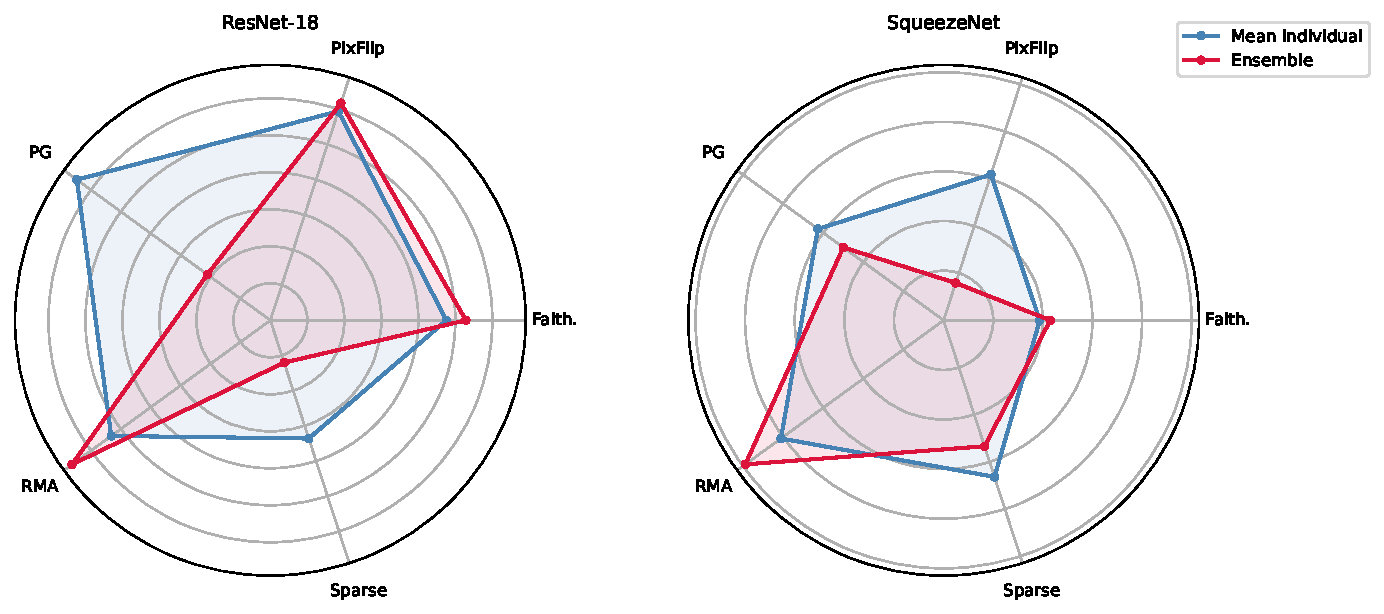
\includegraphics[width=\linewidth]{figures/ensemble_radar.pdf}
    \caption{Per-metric comparison of the NormEnsembleXAI ensemble (crimson)
    against the mean individual attribution method (blue) over the seven
    $M^{*}$ metrics on the full 600 images, normalised per metric against the
    method range and rectified by metric direction, so a larger radius is
    always better. On both models the ensemble trades gains on some metrics
    for losses on others rather than dominating uniformly---which is why its
    scalar effectiveness never exceeds the individual baselines of
    Table~\ref{tab:ensemble}.}
    \label{fig:ensemble-radar}
\end{figure}

%% ========================================================================
\section{Statistical Significance (Contribution~4)}
\label{sec:exp-stats}

The final stage tests whether the observed ranking differences are
statistically significant rather than artefacts of sampling
(Decision~D5). Two complementary procedures are applied to the per-image
effectiveness distributions:

\begin{itemize}
    \item \textbf{Friedman test $+$ Nemenyi post-hoc} across all FAE methods.
    The Friedman test detects whether at least one method differs in mean rank
    across the test images; the Nemenyi post-hoc identifies which pairs differ,
    visualised as a critical-difference (CD) diagram.
    \item \textbf{Wilcoxon signed-rank test} for the paired comparison of
    individual vs.\ NormEnsembleXAI-ensembled attributions
    (Section~\ref{sec:exp-ensemble}), which is inherently paired per image.
\end{itemize}

% Auto-generated by experiments/render_results_tables.py — do not edit.
% Regenerate after each run; \input this file from chapter4_state_observers.tex.
\begin{table}[H]
\centering
\caption{Friedman omnibus test over FAE methods, per model (MQ-discount
weighting; blocks are test images).}
\begin{tabularx}{\linewidth}{llccc}
\toprule
Model & Weighting & Friedman $\chi^2$ & $p$-value & Significant ($\alpha=0.05$) \\
\midrule
ResNet-18  & MQ-discount & 63.54 & $<10^{-3}$ & Yes \\
SqueezeNet  & MQ-discount & 58.14 & $<10^{-3}$ & Yes \\
\bottomrule
\end{tabularx}
\label{tab:friedman}
\end{table}


The Friedman omnibus test rejects the null hypothesis of equal method ranks
decisively on both models (Table~\ref{tab:friedman}): ResNet-18 yields
$\chi^2 = 759.6$ and SqueezeNet $\chi^2 = 1430.3$, both with $p < 10^{-3}$ over
the 600 image blocks under the Autoweighted scheme (uniform:
$\chi^2 = 830.2$ / $1571.3$; MQ-discount: $370.6$ / $1181.9$; likewise
$p < 10^{-3}$). The standardized effect sizes put these in perspective:
Kendall's $W$ indicates small-to-moderate concordance of the per-image
rankings on ResNet-18 ($W = 0.10$--$0.23$ across schemes) and moderate
concordance on SqueezeNet ($0.33$--$0.46$)---the method differences are
unambiguous but far from deterministic at the level of individual images.
Sixteen omnibus and paired tests are recorded for this chapter (including
the single-FC scheme and the auxiliary ensemble pairings); no formal
multiplicity correction is applied, which is immaterial at the observed
$p < 10^{-10}$ but is noted for completeness (the one non-significant
result below is reported as such, not screened out). At least one FAE
method therefore differs significantly in mean rank, so
the Nemenyi post-hoc and CD diagram (Figure~\ref{fig:cd-diagram}) are
warranted; the per-method mean ranks feeding that diagram are in
\texttt{results/cd\_summary.csv}.

\begin{figure}[H]
    \centering
    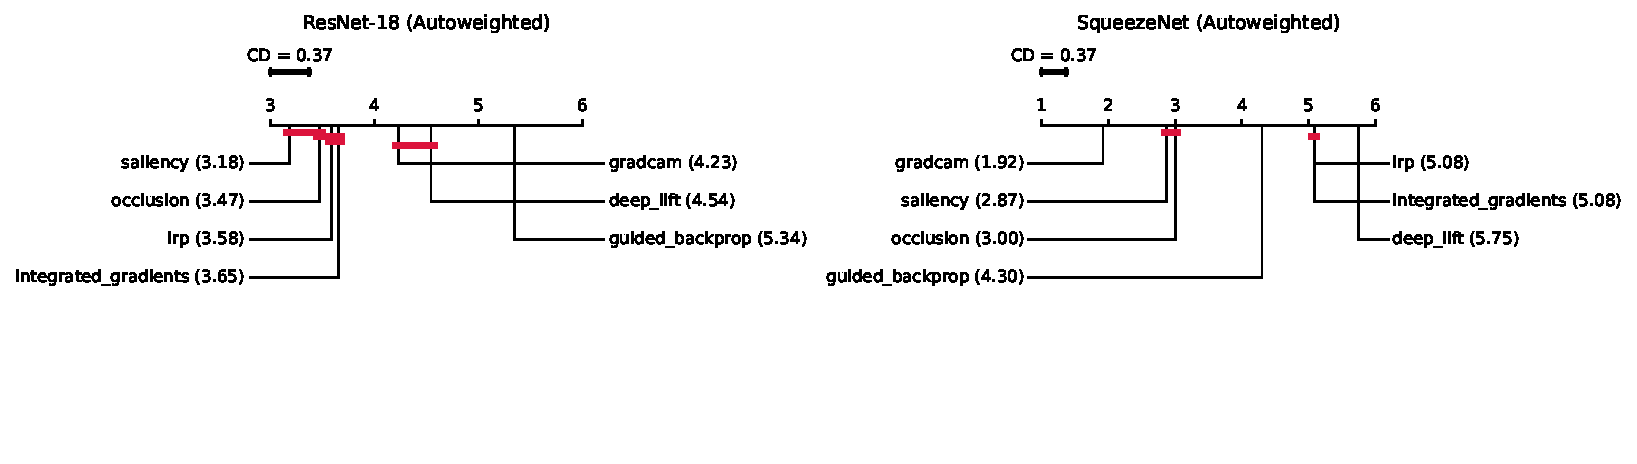
\includegraphics[width=\linewidth]{figures/cd_diagram.pdf}
    \caption{Nemenyi critical-difference diagram over the seven FAE methods
    under the Autoweighted scheme, per model (mean-rank axis; methods joined by
    a crimson bar are not significantly different at $\alpha=0.05$). Occlusion
    leads on ResNet-18 and Grad-CAM on SqueezeNet; the weighting-dependent
    mid-field re-ordering of ResNet-18 (Grad-CAM second under uniform weights,
    fourth here) is visible against the more stable SqueezeNet order.}
    \label{fig:cd-diagram}
\end{figure}

% Auto-generated by experiments/render_results_tables.py — do not edit.
% Regenerate after each run; \input this file from chapter4_state_observers.tex.
\begin{table}[H]
\centering
\caption{Wilcoxon signed-rank tests (paired per image, $n=600$ per model,
pooled normalization): the NormEnsembleXAI-ensembled attribution against the
mean individual method, the best fixed method, and the per-image oracle.
$r$ is the matched-pairs rank-biserial correlation (positive = ensemble
higher). Only the mean-individual rows carry valid inference; see the
text for the post-selection caveat on the other four.}
\small
\begin{tabular}{llcccc}
\toprule
Model & Pair & $W$ & $p$-value & $r$ & Significant \\
\midrule
ResNet-18 & vs.\ mean individual & 62587.0 & $<10^{-3}$ & -0.31 & Yes \\
ResNet-18 & vs.\ best fixed method & 27972.0 & $<10^{-3}$ & -0.69 & Yes \\
ResNet-18 & vs.\ per-image oracle & 562.0 & $<10^{-3}$ & -0.99 & Yes \\
SqueezeNet & vs.\ mean individual & 88718.0 & 0.736 & 0.02 & No \\
SqueezeNet & vs.\ best fixed method & 12004.0 & $<10^{-3}$ & -0.87 & Yes \\
SqueezeNet & vs.\ per-image oracle & 162.0 & $<10^{-3}$ & -1.00 & Yes \\
\bottomrule
\end{tabular}
\label{tab:wilcoxon}
\end{table}


The paired Wilcoxon tests (Table~\ref{tab:wilcoxon}, $n = 600$ per model,
pooled normalization)
quantify the ensemble result of Section~\ref{sec:exp-ensemble}. Against the
\emph{mean} individual method the ensemble is
significantly \emph{worse} on ResNet-18 ($W = 62587$, $p < 10^{-3}$,
rank-biserial $r = -0.31$) and statistically indistinguishable on SqueezeNet
($W = 88718$, $p = 0.74$, $r = 0.02$). Against
the \emph{best fixed} method it is decisively outperformed on both models
($r = -0.69$ and $-0.87$), and against the per-image oracle the losses are
near-total ($r = -0.99$ and $-1.00$). An inferential caveat separates
these comparisons: the mean-individual baseline is selection-free, so its
two tests carry valid $p$-values; the best-fixed and oracle baselines are
\emph{selected on the same 600 images the tests are run on}, so their
$p$-values are post-selection-biased and their four rows are reported as
descriptive effect sizes only---though at $r \le -0.69$ the direction
would survive any reasonable selection correction. The defensible
statistical conclusion is therefore: the Mean ensemble does not beat the
average individual method (significantly worse on ResNet-18, a null on
SqueezeNet), and descriptively it falls far short of every stronger
baseline.

The broader interpretation of these tests is carried into the discussion of
Chapter~\ref{ch:discussion}.
